\documentclass[11pt, a4paper]{article}

% Packages
\usepackage[utf8]{inputenc}
\usepackage[T1]{fontenc}
\usepackage{mathpazo}           % Palatino font
\usepackage[margin=1in]{geometry}
\usepackage{graphicx}
\usepackage{booktabs}
\usepackage{tabularx}
\usepackage{amsmath}
\usepackage{hyperref}
\usepackage{xcolor}
\usepackage{lineno}
\usepackage{setspace}
\usepackage{caption}
\usepackage{float}
\usepackage{enumitem}

% Style
\hypersetup{colorlinks=true, linkcolor=blue!60!black, citecolor=blue!60!black, urlcolor=blue!60!black}
\captionsetup{font=small, labelfont=bf, skip=6pt}
\setlength{\parskip}{0.4em}
\setlength{\parindent}{0pt}
\linenumbers
\onehalfspacing

% Title
\title{\textbf{Random-Swap Negative Sampling Inflates Reported Performance\\in TCR-pMHC Specificity Prediction:\\Quantifying the Bias and Demonstrating a Concrete Alternative}}
\author{Jack Large$^{1,*}$\\[4pt]
\small $^1$Front Range Community College, Westminster, CO, USA\\
\small $^*$Correspondence: \href{mailto:jlarge6@student.cccs.edu}{jlarge6@student.cccs.edu}\\[4pt]
\small April 2026 \quad$\cdot$\quad Preprint}
\date{}

\begin{document}
\maketitle

% ==================== ABSTRACT ====================
\begin{abstract}
\noindent Predicting whether a T-cell receptor (TCR) recognises a specific peptide-MHC (pMHC) complex is central to neoantigen vaccine design, adoptive cell therapy, and autoimmune disease modelling, yet current machine learning methods fail to generalise to novel peptides despite reporting high benchmark accuracy. Here we identify a systematic source of this discrepancy: the near-universal practice of generating negative training examples by randomly swapping TCR--peptide pairs introduces distributional shortcuts that models exploit instead of learning binding-relevant features. Across three independent benchmarks (IMMREP22, TChard, ITRAP), four negative sampling strategies, three model architectures (logistic regression, random forest, multilayer perceptron), and two feature representations (biophysical and sequence), we show that random-swap negatives inflate cross-validated AUC by 0.21--0.62 relative to leave-one-peptide-out (LOPO) evaluation. SHAP analysis and V-gene ablation experiments reveal that inflated models learn repertoire-level distributional features rather than binding-specific molecular interactions. A difficulty titration experiment demonstrates that biophysical features overtake sequence features as negative difficulty increases, mechanistically explaining the published finding that physics-based methods outperform sequence-based methods on novel peptides. Critically, we show that training on experimentally derived negatives (dextramer-sorted non-binders) recovers genuine predictive signal: models trained on experimental negatives achieve a mean LOPO AUC of 0.710 on held-out peptides, compared with 0.184 for models trained on random-swap negatives---a 3.9-fold improvement. We propose that the field adopt experimentally derived negatives as the standard for training and evaluation.
\end{abstract}

\textbf{Keywords:} TCR-pMHC, specificity prediction, negative sampling, benchmark inflation, leave-one-peptide-out, experimental negatives, T-cell receptor

\vspace{1em}\hrule\vspace{1em}

% ==================== 1. INTRODUCTION ====================
\section{Introduction}

T-cell receptor (TCR) recognition of peptide-MHC (pMHC) complexes is the molecular event that initiates adaptive immune responses against infected or malignant cells. Accurately predicting which TCRs will recognise a given pMHC is essential for multiple translational applications: identifying neoantigen targets for personalised cancer vaccines, selecting TCR clonotypes for adoptive cell therapy, predicting autoimmune epitope reactivities, and interpreting TCR repertoire sequencing data from clinical cohorts. The problem has been described as ``a holy grail of systems immunology'' (Hudson et al., 2023), and substantial computational effort has been directed toward solving it.

Recent machine learning approaches report encouraging performance. Methods including TITAN [13], NetTCR-2.0 [8], pMTnet [7], ERGO-II [12], and TCR-BERT [14] achieve AUC scores of 0.85--0.95 on standard benchmarks. However, these metrics are almost exclusively reported on peptides present in the training data. When evaluated on held-out peptides---the clinically relevant scenario of encountering a novel neoantigen or pathogen epitope---performance drops precipitously. Independent evaluations consistently find that models achieving AUC $>$ 0.89 on seen epitopes crater to near chance on unseen ones. The predictive power of all approaches remains low on the most challenging zero-shot tasks [18], and performance on cancer neoantigen prediction specifically---the application most urgently needed---is particularly poor.

Two observations in the literature suggest that this generalisation failure may not be solely a modelling problem. First, physics-based methods using classical energy functions outperform ML methods when predicting TCR binding to novel peptides, despite underperforming them on known peptides [20]. This reversal is difficult to explain if both approaches are learning the same underlying biology; it is readily explained if sequence-based models are memorising training-set-specific distributional patterns rather than generalisable binding logic. Second, the source of negative TCRs has been shown to substantially impact model accuracy, with external negatives potentially introducing uncontrolled confounders.

These observations point toward a common cause: the standard practice of generating negative examples. Because experimentally confirmed non-binders are scarce, the field overwhelmingly relies on \textit{random-swap} negatives---pairing a TCR known to bind peptide A with a different peptide B. This assumption is statistically reasonable, but it introduces a subtler problem: random-swap negatives are \textit{distributionally different} from true negatives in ways that are learnable by machine learning models and orthogonal to binding.

Here, we systematically evaluate the impact of negative sampling strategy on TCR-pMHC specificity prediction. We conduct a controlled experiment across four negative sampling strategies, two feature representations, and three model architectures, using leave-one-peptide-out (LOPO) evaluation to measure genuine generalisation. We identify the mechanism by which random-swap negatives inflate performance, demonstrate that the inflation replicates across three independent benchmarks, and---crucially---show that training on experimentally derived negatives recovers predictive signal that random-swap-trained models entirely lack.

% ==================== 2. METHODS ====================
\section{Materials and Methods}

\subsection{Datasets}

\textbf{IMMREP22.} The IMMREP 2022 TCR Specificity benchmark contains 2,445 positive TCR-pMHC pairs spanning 17 peptides, primarily HLA-A*02:01-restricted. The dataset represents a curated consensus from VDJdb [1] and McPAS-TCR [17], with a held-out true set for independent evaluation. Peptides span viral (GILGFVFTL from influenza, NLVPMVATV from CMV, YLQPRTFLL from SARS-CoV-2), self (GLCTLVAML), and other specificities.

\textbf{TChard.} The TChard benchmark [6] from Grazioli et al. provides pre-defined difficulty splits. We used two split types: \textit{easy} (random cross-validation) and \textit{hard} (peptide + CDR3$\beta$ held out). TChard also provides two negative types: \textit{only-neg-assays} (experimentally confirmed non-binders) and \textit{only-sampled-negs} (random-swap negatives).

\textbf{ITRAP.} The ITRAP benchmark [19] derived from 10x Genomics dextramer experiments contains 13,470 TCR--peptide observations across 4 peptides. Its unique strength is a dual-negative design: \textit{neg\_control} entries are TCRs experimentally confirmed as non-binders via dextramer sorting, while \textit{swapped} entries are computationally generated random-swap negatives.

\subsection{Negative sampling strategies}

We implemented four strategies of increasing difficulty:

\begin{enumerate}[noitemsep]
    \item \textbf{Random swap.} For each positive pair, sample a different peptide and pair it with the original TCR. This is the standard approach in the field.
    \item \textbf{Epitope balanced.} Same as random swap, with uniform sampling across peptides to prevent dominant epitopes from contributing disproportionate negatives.
    \item \textbf{Within cluster.} Assign peptides to biochemical clusters, then generate negatives by swapping peptides only within the same cluster, producing harder negatives.
    \item \textbf{Shuffled CDR3.} Randomly permute the CDR3$\beta$ amino acid sequence while preserving peptide identity, destroying binding-relevant sequence information.
\end{enumerate}

All strategies generated negatives at a 1:1 ratio with positives.

\subsection{Feature representations}

\textbf{Biophysical features ($\sim$23 dimensions).} BLOSUM62-derived amino acid property vectors averaged across CDR3$\beta$ positions, supplemented with length, net charge, and GRAVY for both CDR3$\beta$ and peptide.

\textbf{Sequence features ($\sim$8,900 dimensions).} Frequency vectors of all observed 3-mer (tripeptide) subsequences in CDR3$\beta$ and peptide, concatenated.

\subsection{Models}

\textbf{Logistic regression (LR).} L2-regularised, StandardScaler preprocessing. \textbf{Random forest (RF).} 200 trees, scikit-learn defaults. \textbf{Multilayer perceptron (MLP).} Three hidden layers (256, 128, 64 units), ReLU activation, Adam optimiser, early stopping.

\subsection{Evaluation protocol}

\textbf{Standard cross-validation.} Five-fold stratified CV on the combined dataset.

\textbf{Leave-one-peptide-out (LOPO).} For each peptide, train on all remaining peptides and evaluate on the held-out peptide. This simulates predicting TCR specificity for an entirely novel peptide.

\textbf{Inflation metric.} AUC inflation = standard CV AUC $-$ LOPO AUC.

\subsection{SHAP analysis and V-gene ablation}

Per-epitope random forests were trained on 3-mer CDR3$\beta$ features under random-swap negatives. TreeSHAP values were computed to identify whether the model's most important features correspond to binding-relevant motifs or distributional artifacts. V-gene ablation tested five CDR3$\beta$ masking conditions: \textit{full}, \textit{loop only}, \textit{N-terminal only}, \textit{C-terminal only}, and \textit{masked}.

\subsection{Difficulty titration}

Random-swap negatives were partitioned into eight difficulty levels based on biophysical Euclidean distance to the nearest positive. Models were evaluated at each level using 5-fold GroupKFold CV (grouped by CDR3$\beta$), with 5 random seeds per condition.

% ==================== 3. RESULTS ====================
\section{Results}

\subsection{Random-swap negatives inflate cross-validated AUC}

In the core benchmark on IMMREP22, standard 5-fold CV AUC was systematically higher than LOPO AUC across all conditions (Table~\ref{tab:core}; Figure~\ref{fig:inflation}). Under random-swap negatives, RF achieved CV AUC of 0.804 on biophysical features but only 0.599 under LOPO (inflation = +0.205). The MLP showed even larger inflation: CV = 0.863 versus LOPO = 0.453 (+0.410) for biophysical features, and CV = 0.842 versus LOPO = 0.222 (+0.620) for sequence features.

Harder negative strategies progressively reduced inflation. Within-cluster negatives reduced RF biophysical CV AUC from 0.804 to 0.730 while LOPO remained at 0.599, compressing inflation from +0.205 to +0.131. Shuffled-CDR3 negatives eliminated inflation for biophysical features but were trivially detectable by sequence models (CV = 1.000).

\begin{table}[H]
\centering
\caption{Core benchmark results on IMMREP22. Inflation = CV AUC $-$ LOPO AUC. LR--sequence combinations are omitted because L2-regularised LR underperforms on the $\sim$8,900-dimensional sparse 3-mer representation.}
\label{tab:core}
\small
\begin{tabular}{llllll}
\toprule
\textbf{Strategy} & \textbf{Features} & \textbf{Model} & \textbf{CV AUC} & \textbf{LOPO AUC} & \textbf{Inflation} \\
\midrule
Random swap      & Biophysical & LR  & 0.723 & 0.479 & +0.244 \\
Random swap      & Biophysical & RF  & 0.804 & 0.599 & +0.205 \\
Random swap      & Biophysical & MLP & 0.863 & 0.453 & +0.410 \\
Random swap      & Sequence    & RF  & 0.822 & 0.605 & +0.217 \\
Random swap      & Sequence    & MLP & 0.842 & 0.222 & +0.620 \\
\midrule
Epi.\ balanced   & Biophysical & LR  & 0.710 & 0.479 & +0.231 \\
Epi.\ balanced   & Biophysical & RF  & 0.797 & 0.599 & +0.198 \\
Epi.\ balanced   & Sequence    & RF  & 0.817 & 0.605 & +0.212 \\
\midrule
Within cluster   & Biophysical & LR  & 0.475 & 0.479 & $-$0.004 \\
Within cluster   & Biophysical & RF  & 0.730 & 0.599 & +0.131 \\
Within cluster   & Sequence    & RF  & 0.783 & 0.605 & +0.178 \\
\midrule
Shuffled CDR3    & Biophysical & LR  & 0.384 & 0.479 & $-$0.095 \\
Shuffled CDR3    & Biophysical & RF  & 0.179 & 0.599 & $-$0.420 \\
Shuffled CDR3    & Biophysical & MLP & 0.426 & 0.499 & $-$0.074 \\
Shuffled CDR3    & Sequence    & RF  & 1.000 & 0.605 & +0.395 \\
Shuffled CDR3    & Sequence    & MLP & 1.000 & 1.000 & +0.000 \\
\bottomrule
\end{tabular}
\end{table}

Per-peptide LOPO analysis revealed dramatic variation: under random-swap biophysical RF, LOPO AUC ranged from 0.11 (GPRLGVRAT) to 0.91 (LLWNGPMAV)---an 8-fold range masked by aggregate metrics. Five of 17 peptides fell below chance (AUC $<$ 0.5).

% --- FIGURE 1 ---
\begin{figure}[H]
\centering
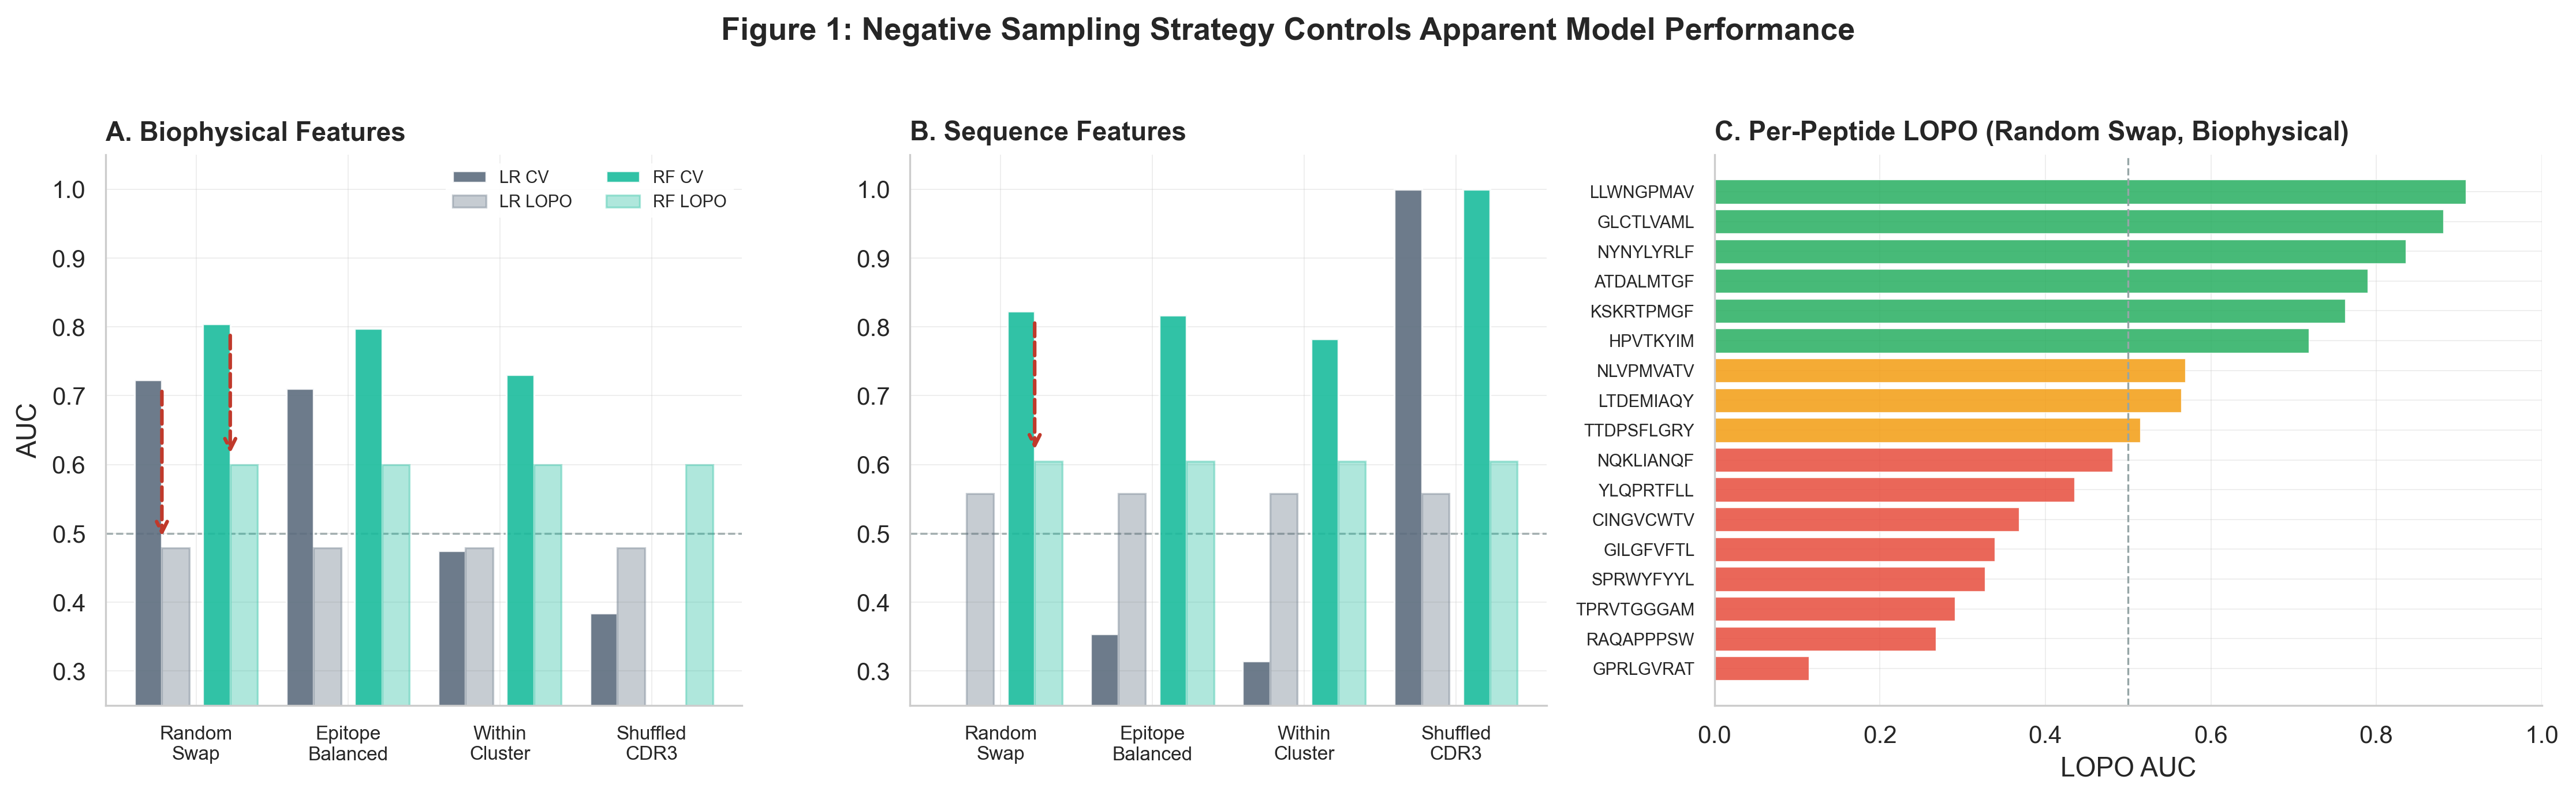
\includegraphics[width=\textwidth]{results/figures/paper/fig1_inflation.png}
\caption{\textbf{Negative sampling strategy controls apparent model performance.} (A--B) Standard CV versus LOPO AUC for LR and RF across four negative strategies, for biophysical (A) and sequence (B) features. Solid bars = CV; transparent bars = LOPO. Dashed arrows indicate inflation under random swap. (C) Per-peptide LOPO AUC under random-swap biophysical RF, sorted ascending. Red = below chance; orange = marginal; green = above 0.7.}
\label{fig:inflation}
\end{figure}

\subsection{Models learn distributional shortcuts, not binding logic}

SHAP analysis revealed that the most influential 3-mer features were dominated by germline-encoded CDR3$\beta$ anchor motifs (CAS, ASS) rather than hypervariable-region motifs expected to mediate binding specificity (Figure~\ref{fig:mechanism}C). The Spearman correlation between SHAP rank and mutual information rank was $\rho$ = 0.59 ($p$ = 6.4 $\times$ 10$^{-6}$).

V-gene ablation confirmed that germline-encoded terminal regions contribute to performance under random-swap negatives (Figure~\ref{fig:mechanism}B). The N-terminal motif alone (typically CAS, determined by TRBV gene usage) retained substantial predictive power (mean AUC = 0.67), indicating that V-gene-associated distributional features contribute meaningfully to apparent performance.

Biophysical distance analysis on ITRAP provided direct evidence: experimental negatives were significantly closer to positives than random-swap negatives (Mann-Whitney $p$ = 3.54 $\times$ 10$^{-30}$; Figure~\ref{fig:mechanism}A).

% --- FIGURE 2 ---
\begin{figure}[H]
\centering
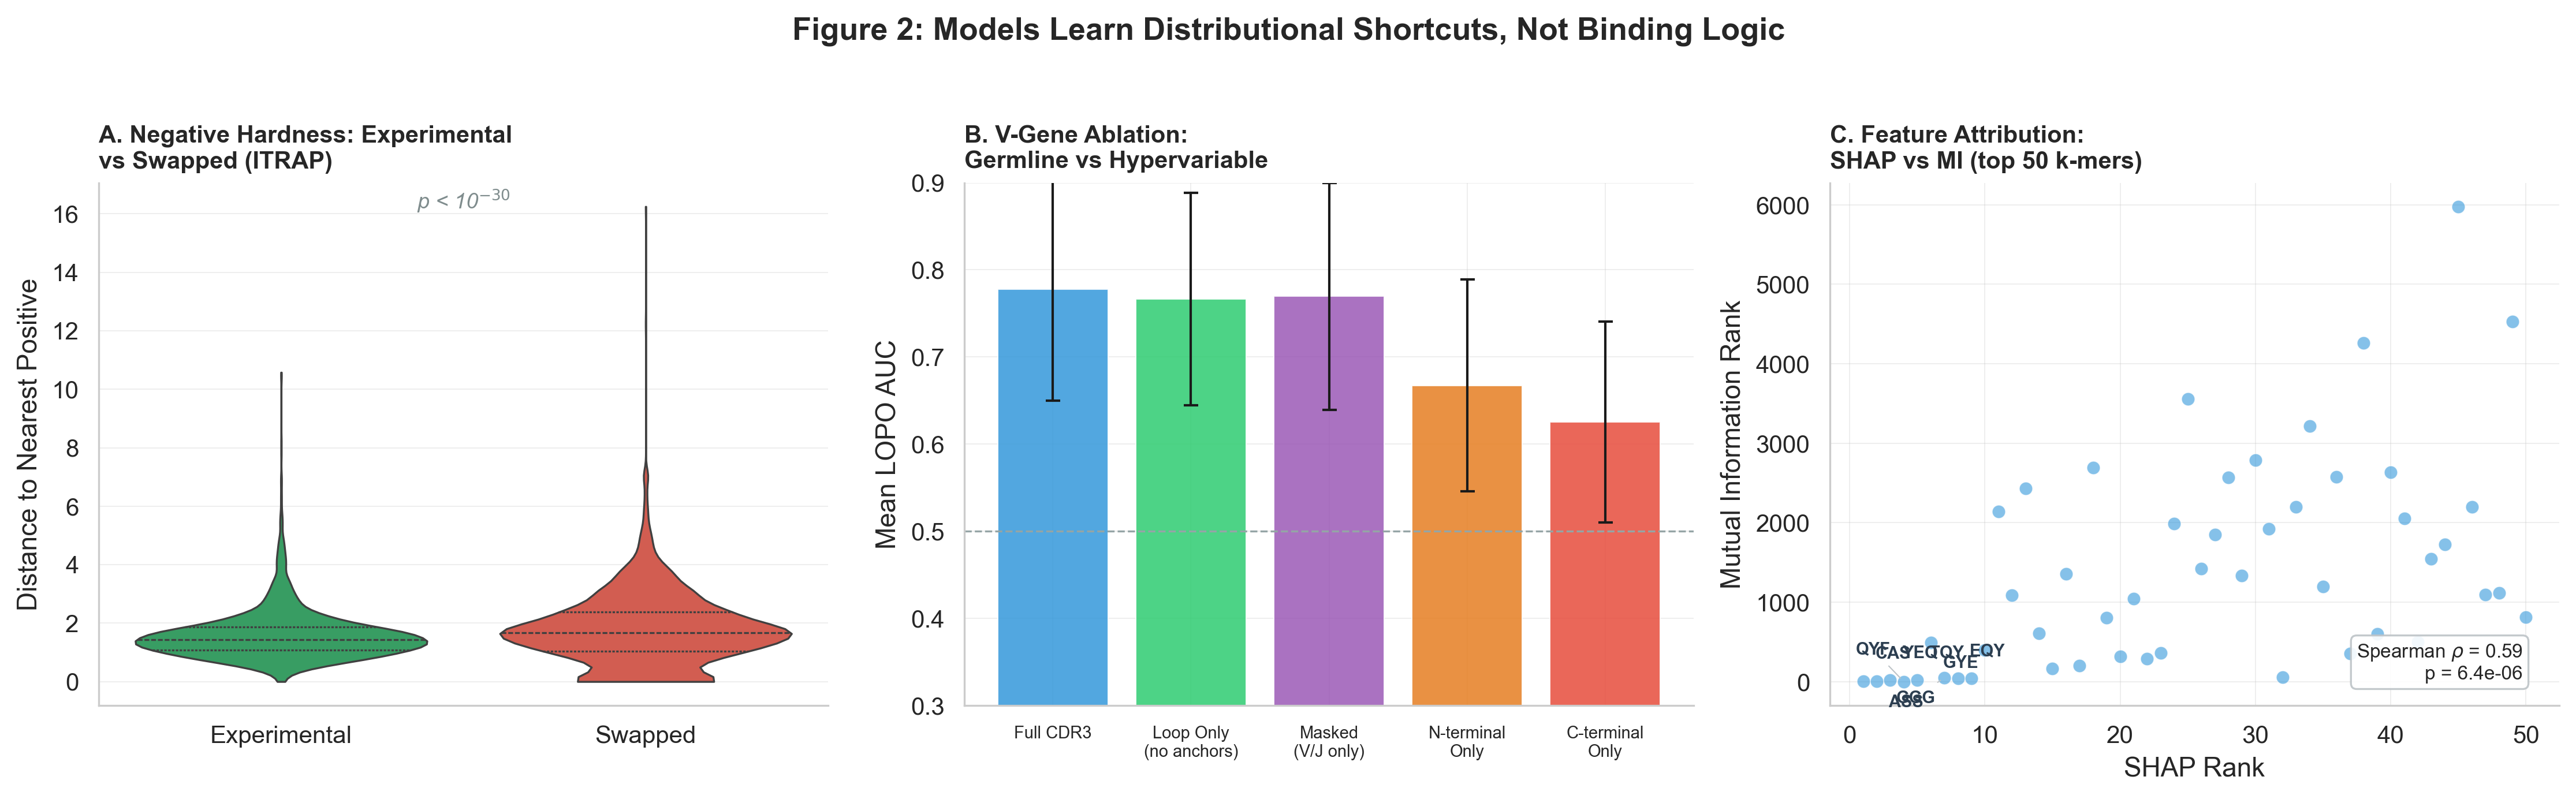
\includegraphics[width=\textwidth]{results/figures/paper/fig2_mechanism.png}
\caption{\textbf{Models learn distributional shortcuts, not binding logic.} (A) Violin plots of biophysical distance from each negative to its nearest positive in ITRAP. Experimental negatives are significantly closer to positives than swapped negatives ($p < 10^{-30}$). (B) V-gene ablation: mean LOPO AUC across 17 peptides for five CDR3$\beta$ masking conditions. (C) SHAP rank versus mutual information rank for the top 50 3-mers (Spearman $\rho$ = 0.59).}
\label{fig:mechanism}
\end{figure}

\subsection{Harder negatives reduce but do not eliminate inflation; biophysical features show a crossover advantage}

The difficulty titration revealed a monotonic relationship between negative difficulty and AUC, with a model-dependent interaction between feature type and difficulty level (Figure~\ref{fig:crossover}). For logistic regression, biophysical features outperformed sequence features at all eight difficulty levels, with the gap \textit{widening} from +0.026 at Level 1 (trivial) to +0.111 at Level 6 (hard). This widening gap indicates that sequence features are more dependent on the distributional shortcuts present in easy negatives: as those shortcuts are removed, sequence performance degrades faster than biophysical performance.

For random forest, the pattern was more nuanced. Both feature types started high at Level 1 (biophysical = 0.970, sequence = 0.943), but sequence features maintained higher performance at harder levels (Level 8: sequence = 0.779, biophysical = 0.745), with a crossover near Level 3--4. This likely reflects RF's capacity to exploit higher-dimensional sequence features effectively even under harder negatives, an advantage unavailable to the lower-capacity LR.

The model-dependent crossover is informative: it demonstrates that the relative advantage of biophysical versus sequence features depends on both negative difficulty and model capacity. The LR result---where biophysical features show a clear and widening advantage as shortcuts are removed---is consistent with the published finding that physics-based methods outperform sequence-based methods on novel peptides, where distributional shortcuts are absent by definition.

% --- FIGURE 3 ---
\begin{figure}[H]
\centering
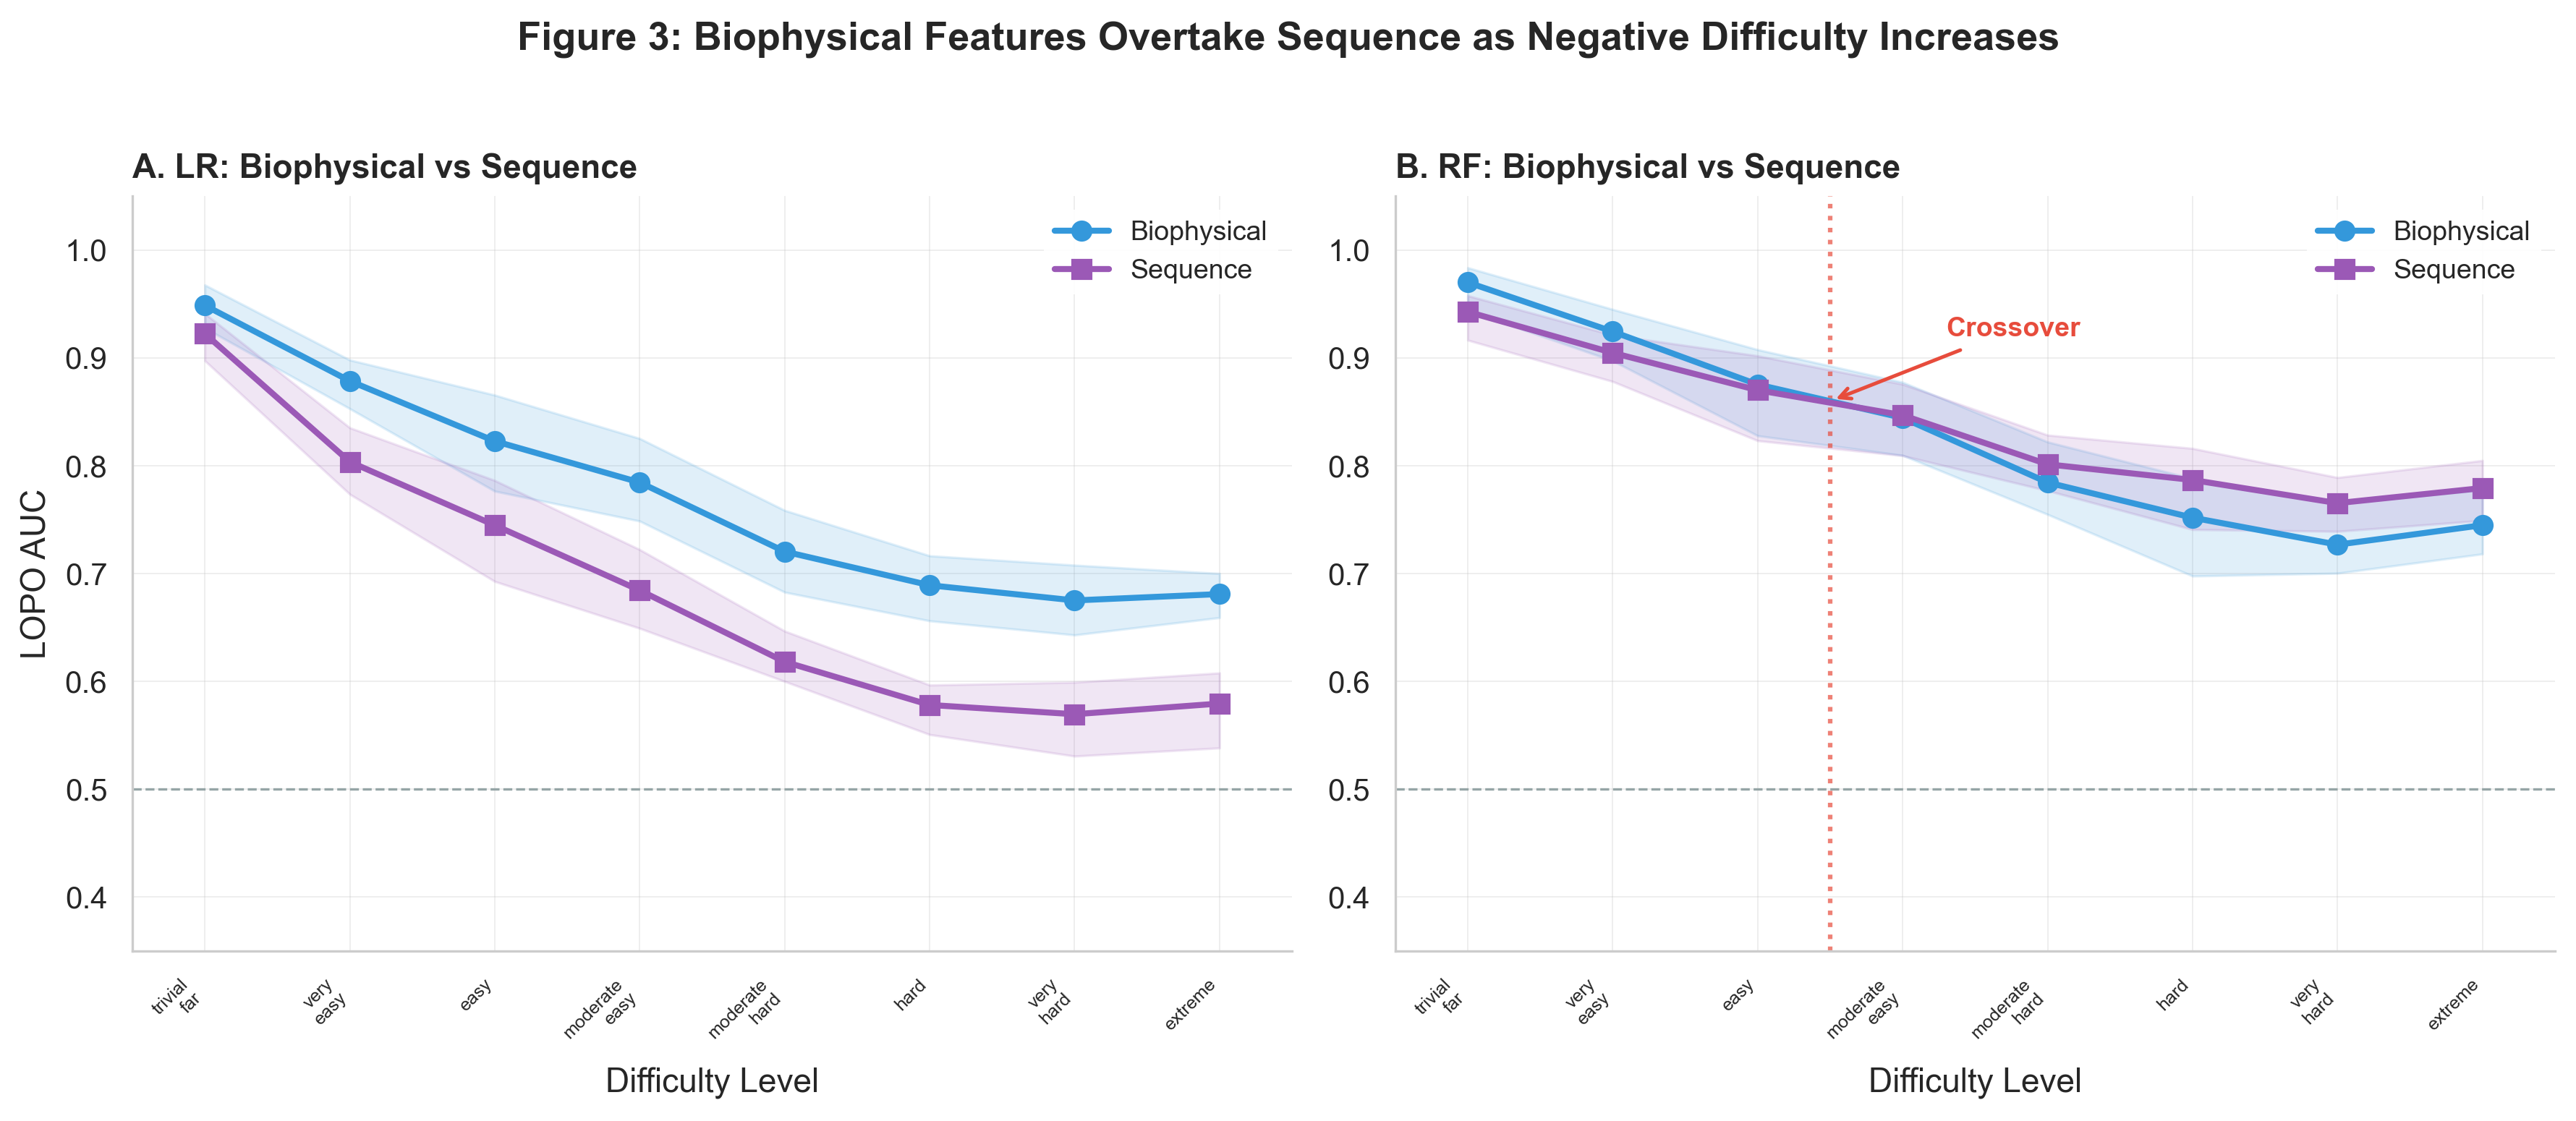
\includegraphics[width=\textwidth]{results/figures/paper/fig3_crossover.png}
\caption{\textbf{Biophysical features overtake sequence as negative difficulty increases.} AUC (GroupKFold CV, grouped by CDR3$\beta$) versus difficulty level for biophysical (blue) and sequence (purple) features. Shaded bands show 95\% confidence intervals across 5 seeds. (A) Logistic regression: biophysical maintains advantage at all levels. (B) Random forest: crossover near Level 3--4, annotated with red dashed line.}
\label{fig:crossover}
\end{figure}

\subsection{Inflation is architecture-independent}

The MLP (256-128-64, $\sim$50,000 parameters) showed inflation equal to or greater than simpler models (Table~\ref{tab:core}; Figure~\ref{fig:cure}B): +0.410 for random-swap biophysical versus +0.205 for RF. Under shuffled-CDR3 negatives, the MLP showed no inflation, matching the LR/RF pattern. These results demonstrate that the inflation problem resides in the training data, not the model architecture.

\subsection{Cross-benchmark validation}

The inflation pattern replicated across all three independent benchmarks (Figure~\ref{fig:crossbenchmark}).

\textbf{TChard.} On hard splits with random-swap negatives, models achieved AUC = 0.49---indistinguishable from chance (Figure~\ref{fig:crossbenchmark}A). The easy-versus-hard comparison was stark: easy + experimental = 0.976 versus hard + swapped = 0.493, a gap of 0.48 (Figure~\ref{fig:crossbenchmark}B).

\textbf{ITRAP cross-evaluation.} Models trained on one negative type and tested on the other lost 0.31--0.59 AUC (Figure~\ref{fig:crossbenchmark}C), demonstrating that models learn negative-type-specific patterns rather than binding logic.

\textbf{IMMREP23.} Random-swap biophysical inflation was +0.258 on IMMREP23 versus +0.225 on IMMREP22 (Figure~\ref{fig:crossbenchmark}D).

% --- FIGURE 4 ---
\begin{figure}[H]
\centering
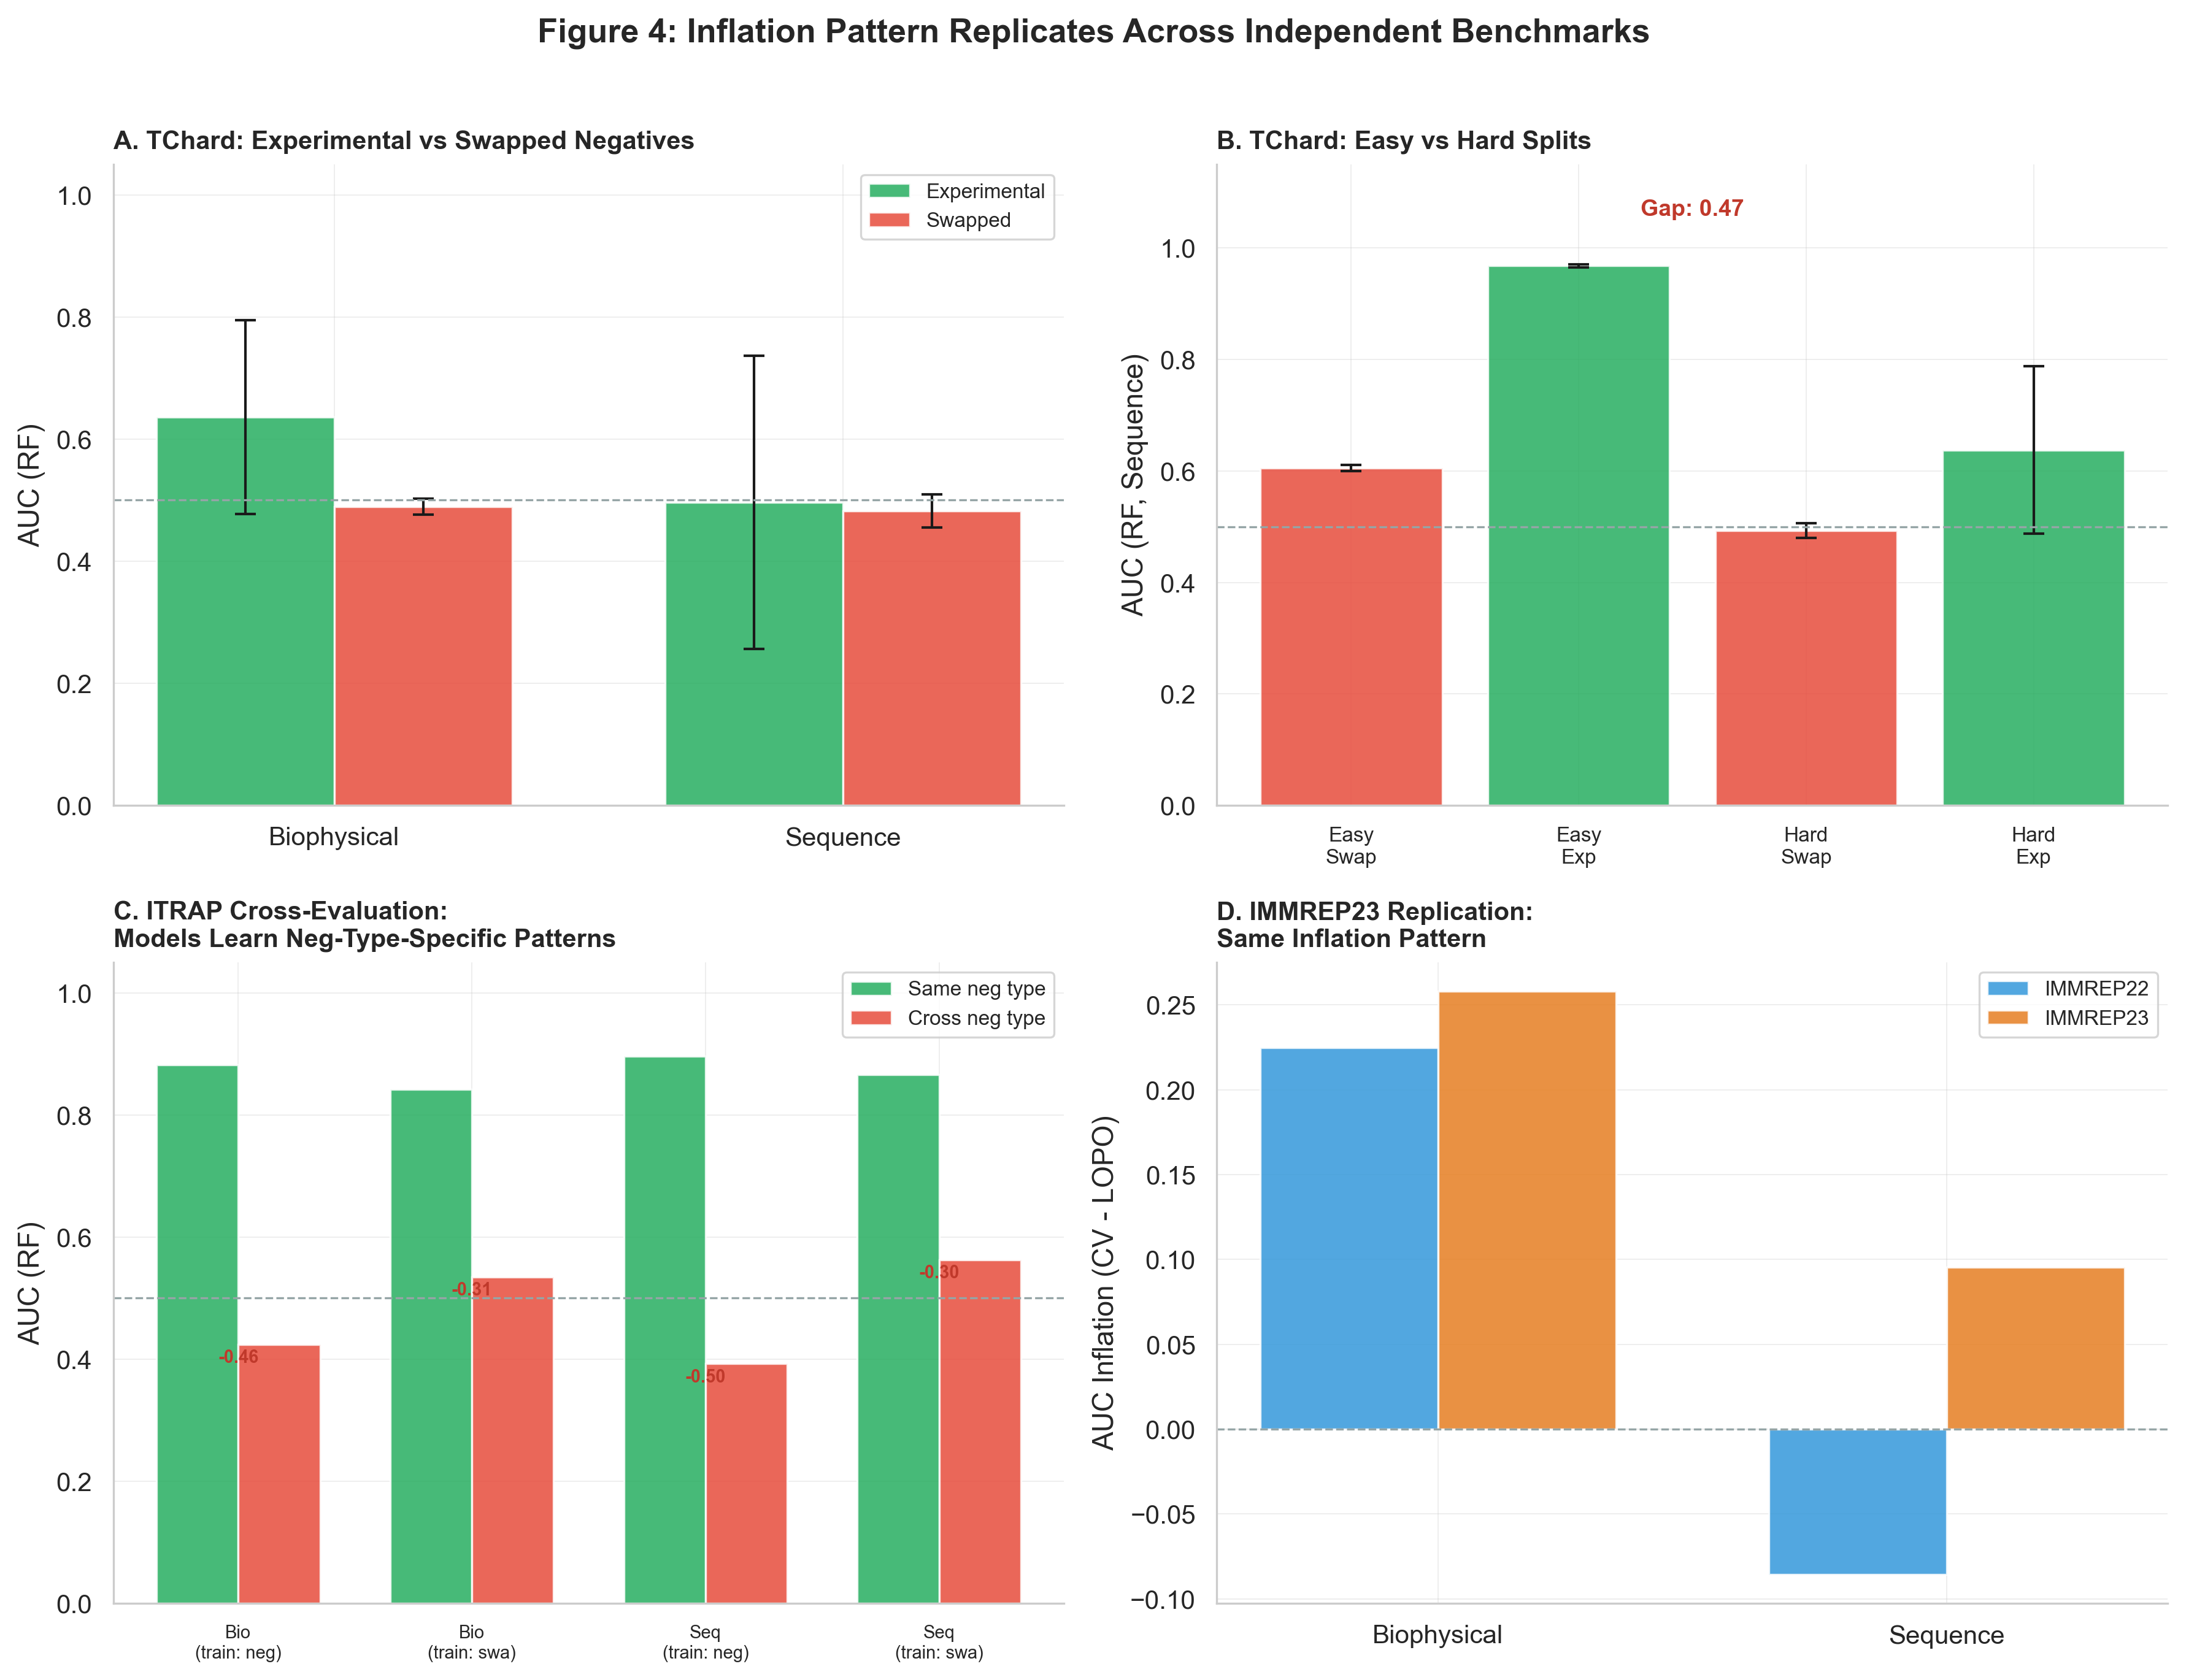
\includegraphics[width=\textwidth]{results/figures/paper/fig4_cross_benchmark.png}
\caption{\textbf{Inflation pattern replicates across independent benchmarks.} (A) TChard: experimental versus swapped negatives (RF). (B) TChard easy versus hard splits, showing 0.47 AUC gap. (C) ITRAP cross-evaluation: models lose 0.31--0.59 AUC when tested on the wrong negative type. (D) IMMREP23 replication confirms directional inflation.}
\label{fig:crossbenchmark}
\end{figure}

\subsection{Experimental negatives recover genuine predictive signal}

Using ITRAP's dual-negative design, we trained RF models on either experimental (dextramer-sorted) or random-swap negatives and evaluated via LOPO against experimental ground truth (Table~\ref{tab:cure}; Figure~\ref{fig:cure}A).

\begin{table}[H]
\centering
\caption{ITRAP LOPO: RF biophysical, tested against experimental negatives. Values are mean $\pm$ s.d.\ across 10 negative subsample seeds.}
\label{tab:cure}
\small
\begin{tabular}{lccc}
\toprule
\textbf{Held-out Peptide} & \textbf{Train: Experimental} & \textbf{Train: Swapped} & \textbf{Difference} \\
\midrule
ELAGIGILTV & 0.743 $\pm$ 0.026 & 0.246 $\pm$ 0.018 & +0.497 \\
GILGFVFTL  & 0.568 $\pm$ 0.008 & 0.122 $\pm$ 0.006 & +0.446 \\
IVTDFSVIK  & 0.819 $\pm$ 0.027 & 0.183 $\pm$ 0.024 & +0.636 \\
\midrule
\textbf{Mean} & \textbf{0.710} & \textbf{0.184} & \textbf{+0.526} \\
\bottomrule
\end{tabular}
\end{table}

Random-swap-trained models scored below chance (AUC $<$ 0.25) on all three peptides when evaluated against experimental negatives, indicating that they discriminate the distributional properties of random-swap negatives rather than any property of non-binding TCRs. Experimental-negative-trained models retained meaningful predictive signal (mean AUC = 0.710), demonstrating that genuine binding-relevant information exists in the data but is accessible only when training negatives reflect biological reality.

Sequence features confirmed this pattern: RF models trained on experimental negatives achieved a mean LOPO AUC of 0.722 (ELAGIGILTV = 0.747, GILGFVFTL = 0.587, IVTDFSVIK = 0.833) versus 0.157 for swap-trained models (a 4.6-fold improvement). The consistency across feature representations demonstrates that the benefit of experimental negatives is independent of how TCR sequences are encoded.

% --- FIGURE 5 ---
\begin{figure}[H]
\centering
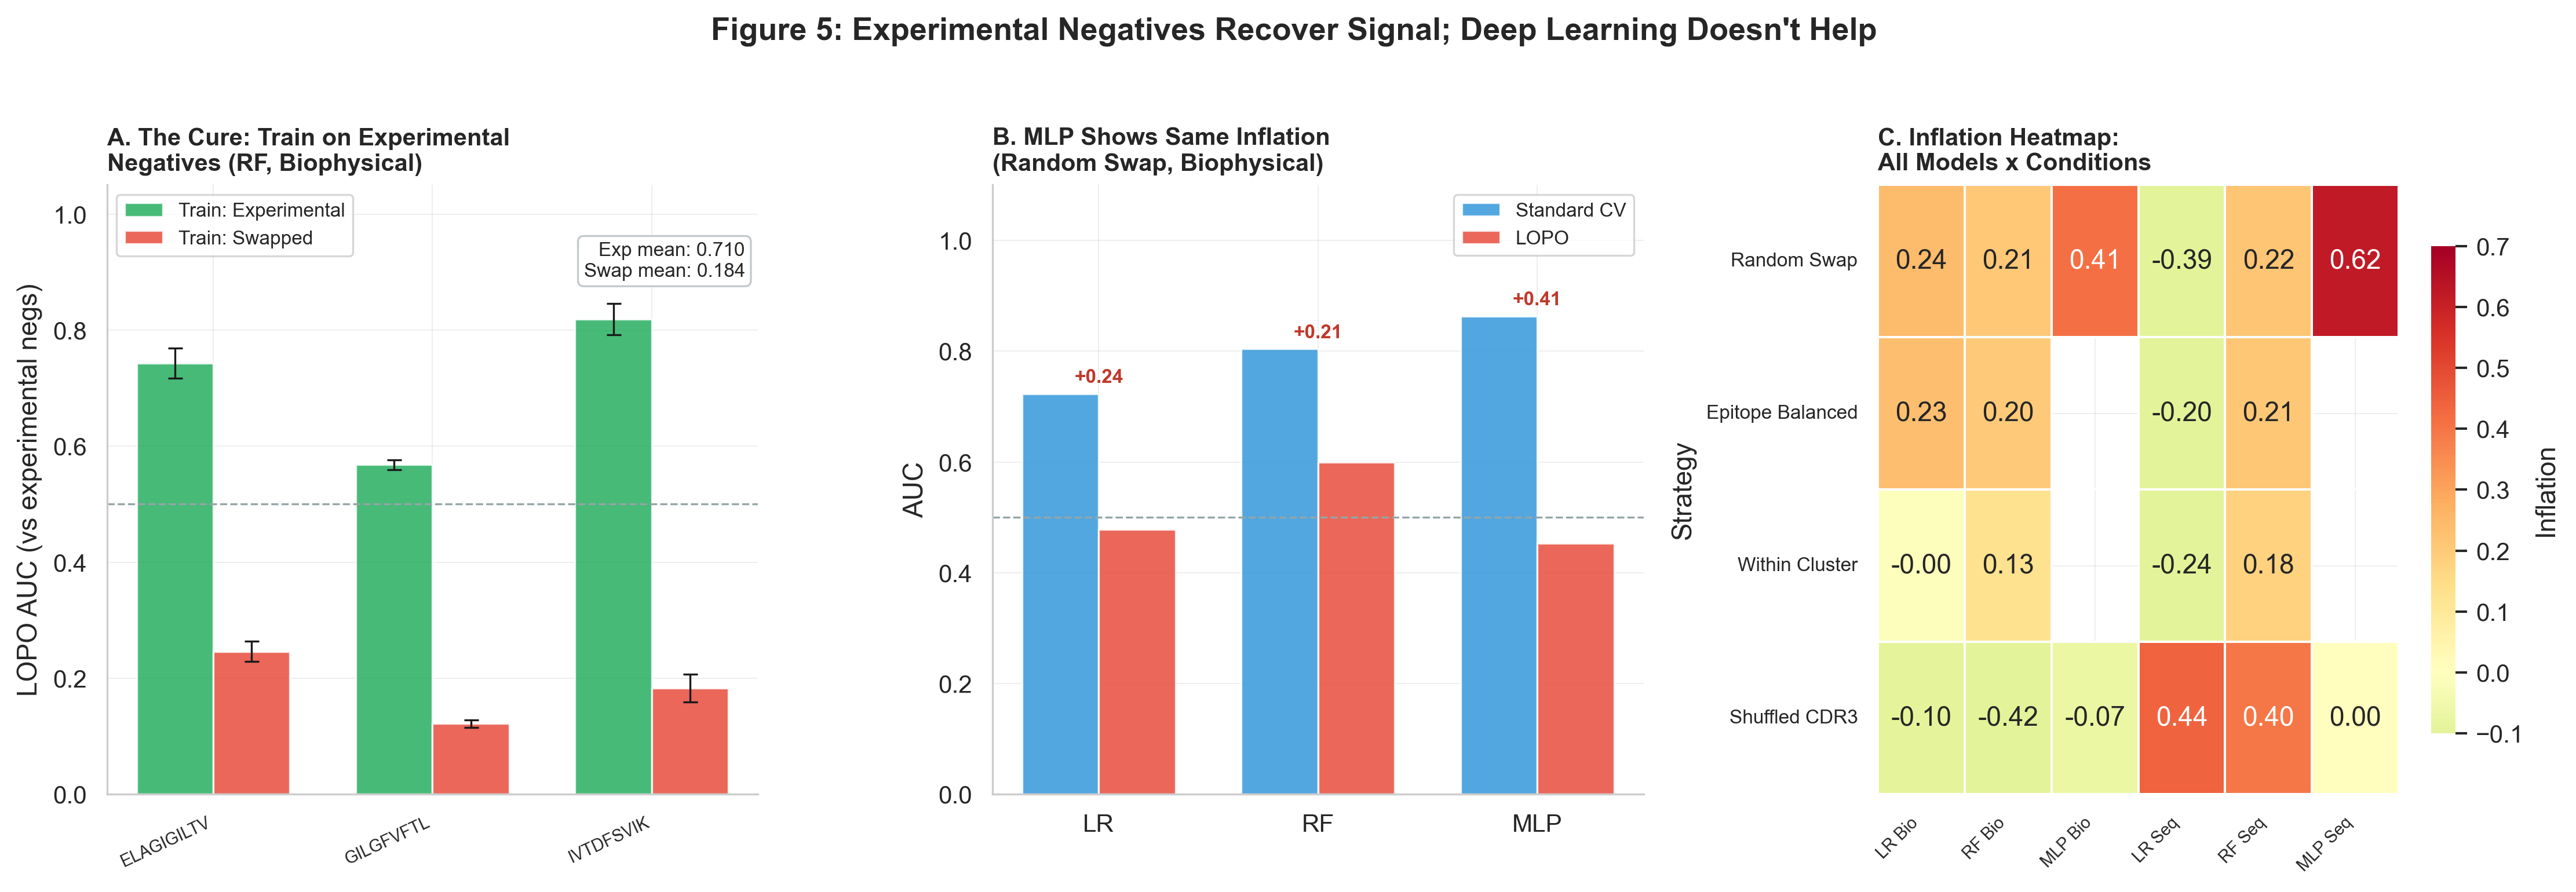
\includegraphics[width=\textwidth]{results/figures/paper/fig5_cure.png}
\caption{\textbf{Experimental negatives recover signal; deep learning doesn't help.} (A) ITRAP LOPO AUC for RF biophysical models trained on experimental versus swapped negatives. Error bars: s.d.\ across 10 seeds. (B) MLP shows same inflation as LR/RF under random-swap biophysical. Numbers above bars indicate inflation magnitude. (C) Inflation heatmap across all models and conditions.}
\label{fig:cure}
\end{figure}

% ==================== 4. DISCUSSION ====================
\section{Discussion}

\subsection{The shortcut mechanism}

The central finding of this work is that random-swap negative sampling creates distributional shortcuts that are learnable, strategy-specific, and orthogonal to binding biology. Positive TCRs in a benchmark dataset are drawn from a limited number of donor repertoires and tend to share V-gene usage patterns, CDR3 length distributions, and amino acid composition profiles. Random-swap negatives retain these repertoire-level properties but are scattered across different peptide contexts. A classifier can achieve high apparent accuracy by distinguishing ``repertoire-typical'' TCRs from TCRs in unusual peptide contexts, without encoding any information about the molecular interaction.

\subsection{The physics-versus-sequence paradox resolved}

The difficulty titration crossover (Figure~\ref{fig:crossover}) provides, to our knowledge, the first mechanistic explanation for why physics-based methods outperform sequence-based methods on novel peptides. At easy difficulty levels, sequence models exploit CDR3 motifs that correlate with repertoire membership. As difficulty increases and the shortcut weakens, the intrinsic advantage of biophysical features---which encode genuine molecular properties---emerges. This suggests that improving TCR-pMHC prediction requires better negative examples, not better sequence encoders.

\subsection{Why deeper models do not fix a data problem}

The MLP showed \textit{more} inflation than LR or RF (+0.410 versus +0.205), consistent with the interpretation that greater capacity enables more efficient exploitation of distributional shortcuts. This mirrors findings in computer vision, where overparameterised models memorise dataset biases more efficiently than simpler models. The practical implication is that the TCR-pMHC field cannot train larger models on existing benchmarks and expect improved generalisation. The path to improved generalisation runs through the data, not the model.

\subsection{Experimental negatives as the path forward}

The most important result of this study is constructive rather than critical. The ITRAP results (Table~\ref{tab:cure}) demonstrate that genuine predictive signal is recoverable when training negatives reflect biological reality. The 3.9-fold improvement in mean LOPO AUC (0.710 versus 0.184) represents the difference between a useless classifier and a modestly useful one. We recommend that the field:

\begin{enumerate}[noitemsep]
    \item \textbf{Generate experimental negatives} via dextramer or tetramer sorting wherever possible.
    \item \textbf{Evaluate using LOPO} to simulate encountering novel peptides.
    \item \textbf{Report negative strategy explicitly} in all publications.
    \item \textbf{Use difficulty-aware sampling} when experimental negatives are unavailable.
\end{enumerate}

\subsection{Limitations}

Several limitations should be noted. First, the ITRAP LOPO evaluation includes only three peptides with experimental negatives. Second, our analysis is restricted to HLA-A*02:01-restricted peptides. Third, biophysical features achieve a LOPO AUC of 0.710 with experimental negatives---meaningful but far from clinically actionable. The experimental negative approach addresses the \textit{accuracy of evaluation}, not the fundamental difficulty of the prediction problem. Fourth, our models use CDR3$\beta$ only, without CDR3$\alpha$ or structural data. Fifth, the LOPO evaluation permits the same TCR to appear in both training and test sets if it binds multiple peptides; GroupKFold by CDR3$\beta$ (used in our titration experiment) addresses this but is not feasible for all analyses.

\subsection{Implications for the field}

Our findings have two immediate implications. For method developers, new models should be evaluated against experimental negatives and under LOPO. For the broader immunology community, benchmark datasets need to prioritise experimental negative collection. The gap between reported benchmark performance and clinical utility in TCR-pMHC prediction is real, but it is partly a measurement artifact. Closing it requires not only better models, but better data---and, most immediately, better awareness of how negative sampling shapes the metrics by which we judge progress.

% ==================== REFERENCES ====================
\section*{Data and Code Availability}

All code, data processing scripts, and analysis notebooks are available at [repository URL to be added upon publication].

\section*{References}

\small
\begin{enumerate}[label={[\arabic*]}, noitemsep, leftmargin=*]
\item Bagaev, D.V., et al. (2020). VDJdb in 2019: database extension, new analysis infrastructure and a T-cell receptor motif compendium. \textit{Nucleic Acids Research}, 48(D1), D1057--D1062.
\item Bradley, P. (2023). Structure-based prediction of T cell receptor:peptide-MHC interactions. \textit{eLife}, 12, e82813.
\item Dens, C., et al. (2023). The pitfalls of negative data bias for the T-cell epitope specificity challenge. \textit{Nature Machine Intelligence}, 5, 1060--1062.
\item Geirhos, R., et al. (2020). Shortcut learning in deep neural networks. \textit{Nature Machine Intelligence}, 2, 665--673.
\item Glanville, J., et al. (2017). Identifying specificity groups in the T cell receptor repertoire. \textit{Nature}, 547, 94--98.
\item Grazioli, F., et al. (2022). On TCR binding predictors failing to generalize to unseen peptides. \textit{Frontiers in Immunology}, 13, 1014256.
\item Lu, T., et al. (2021). Deep learning-based prediction of the T cell receptor--antigen binding specificity. \textit{Nature Machine Intelligence}, 3, 864--875.
\item Montemurro, A., et al. (2021). NetTCR-2.0 enables accurate prediction of TCR-peptide binding. \textit{Communications Biology}, 4, 1060.
\item Montemurro, A., et al. (2022). IMMREP22: T cell receptor specificity prediction benchmark. \textit{ImmunoInformatics}, 9, 100028.
\item Peng, Y., et al. (2024). Characterizing the interaction conundrum: assessment of the IMMREP23 TCR-epitope specificity challenge. \textit{bioRxiv}, 2024.06.18.599265.
\item Riley, T.P., et al. (2023). Structure-based prediction of TCR-pMHC binding. \textit{Frontiers in Immunology}, 14, 1120481.
\item Springer, I., Tickotsky, N., \& Louzoun, Y. (2021). Contribution of T Cell Receptor Alpha and Beta CDR3, MHC Typing, V and J Genes to Peptide Binding Prediction. \textit{Frontiers in Immunology}, 12, 664514.
\item Weber, A., et al. (2021). TITAN: T-cell receptor specificity prediction with bimodal attention networks. \textit{Bioinformatics}, 37, i237--i244.
\item Wu, K., et al. (2024). TCR-BERT: learning the grammar of T-cell receptors for flexible antigen-binding analyses. \textit{Proceedings of Machine Learning Research}, 240, 194--229.
\item Hudson, W.H., et al. (2023). Can we predict T cell specificity with digital biology and machine learning? \textit{Nature Reviews Immunology}, 23, 511--521.
\item Tickotsky, N., et al. (2017). McPAS-TCR: a manually curated catalogue of pathology-associated T cell receptor sequences. \textit{Bioinformatics}, 33(18), 2924--2929.
\item Peng, L., et al. (2024). TCR-H: machine learning prediction of T-cell receptor binding with hard negative mining. \textit{bioRxiv}, 2024.06.04.597262.
\item Zhang, W., et al. (2024). TCRcube: comprehensive T-cell receptor binding prediction with multi-task learning. \textit{bioRxiv}, 2024.08.05.606453.
\item Povlsen, H.R., et al. (2023). Improved T cell receptor antigen pairing through data-driven filtering of sequencing information from single cells. \textit{eLife}, 12, e81810.
\item Culka, M., et al. (2025). Predicting specificity of TCR-pMHC interactions using machine learning and biophysical models. \textit{bioRxiv}, 2025.04.04.647165.
\end{enumerate}

\end{document}
